\begin{frame}
	\frametitle{Partikelschwarm Algorithmus}
	
	\section[Algorithmus]{Partikelschwarm Algorithmus}
	Zustandsdaten jedes Partikels:
	\begin{align*}
		x_i: \: \: & \text{aktuelle Position}\\
		v_i: \: \: & \text{aktuelle Geschwindigkeit}\\
		p_i: \: \: & \text{Persönlich beste Position} \\
		l_i: \: \: & \text{Beste Position des Schwarms}
	\end{align*}
	

	Initialisierung:
	\begin{align*}
		x_i(0) &= U(min,max) \\
		v_i(0) &= U(min - x_i(0), max - x_i(0)) \\
		p_i(0) &= x_i(0)
	\end{align*}
	
\end{frame}

\begin{frame}
	\frametitle{Partikelschwarm Algorithmus}
	Geschwindigkeits- und Positions-Update:
	\begin{align*}
		v_i(t+1) &= w v_i(t) \\
				&+ U(0,c_1) \left(p_i(t)-x_i(t) \right) \\
				&+ U(0,c_2) \left(l_i(t)-x_i(t) \right) \\
		x_{i}(t+1) &= x_i(t) + v_i(t+1)
	\end{align*}

	\begin{align*}
		w &: \text{Intertia Weight} \\
		c_1 &: \text{Cognitive Factor} \\
		c_2 &: \text{Social Factor} \\
		U(a,b) &: \text{Random Number between a,b}
	\end{align*}	
\end{frame}

\begin{frame}
	\frametitle{Partikelschwarm Algorithmus}
	Visualisierung
	\begin{figure}[htbp]
		\documentclass{standalone}

\usepackage{tikz}
\usetikzlibrary{arrows,decorations.pathmorphing,positioning,fit,petri}
\usetikzlibrary{calc,intersections,through,backgrounds,graphs}
\usetikzlibrary{patterns,decorations.pathreplacing}

\begin{document}

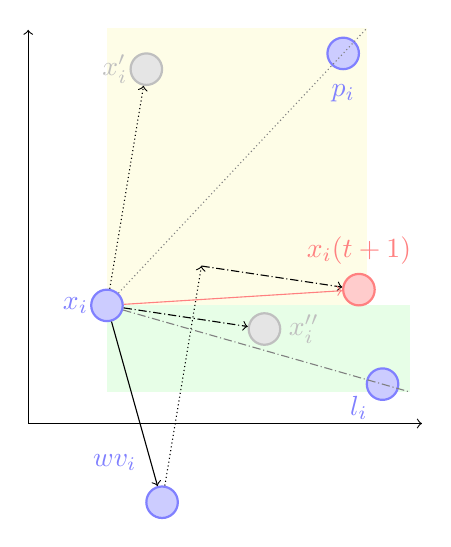
\begin{tikzpicture}
	% Styles
	[
	point/.style={circle,draw=blue!50,fill=blue!20,thick, inner sep=0pt,minimum size=4mm},
	vpoint/.style={circle,draw=gray!50,fill=gray!20,thick, inner sep=0pt,minimum size=4mm},
	endpoint/.style={circle,draw=red!50,fill=red!20,thick, inner sep=0pt,minimum size=4mm},
	]
                      
	% Axis
	\draw[->] (0,0) -- (5,0);
  	\draw[->] (0,0) -- (0,5);
	
	% Shaded Parts
	\fill[gray!10!yellow!10] (1,1.5) rectangle (4.3,5.02);
	\fill[gray!10!green!10] (1,1.5) rectangle (4.85,0.4);

	% Nodes
	\node at (1.5,4.5)	(xi1)	[vpoint]	{};
	\node at (3,1.2)	(xi2)	[vpoint]	{};
	\node at (4,4.7)	(pi)	[point] 	{};
	\node at (4.5,0.5)	(li)	[point] 	{};
	\node at (1.7,-1)	(wvi) [point]	{};
	\node at (1,1.5)	(xi)	[point]	{} 
		edge [->,densely dotted]			(xi1)
		edge[densely dotted,gray]		(4.3,5.02)
		edge[->,densely dashdotted]		(xi2)
		edge[densely dashdotted,gray]	(4.85,0.4);
	\node at (4.2,1.7)	(xit)	[endpoint] {};
	\draw[->] (xi) -- (wvi);
	\draw[->,densely dotted] (wvi)  -- (2.2,2);
	\draw[->,densely dashdotted] (2.2,2) -- (xit);
	\draw[->,red!50]	(xi) -- (xit);

	% Text
	\node[blue!50]		at (0.6,1.5)	{$x_i$};
	\node[gray!50]		at (1.1,4.5) 	{$x'_i$};
	\node[gray!50]		at (3.5,1.2) 	{$x''_i$};
	\node[blue!50]		at (4,4.2)		{$p_i$};
	\node[blue!50]		at (4.2,0.2)	{$l_i$};
	\node[red!50]		at (4.2,2.2)	{$x_i(t+1)$};
	\node[blue!50]		at (1.1,-0.5)	{$wv_i$};

\end{tikzpicture}

\end{document}
	\end{figure}
\end{frame}